\documentclass[11pt,a4paper,oneside]{book}
% We load package by package and set package relevant parameters.
% Topics are summarized later
%%%%%%%%%%%%%%%%%%%%%%%%%%%%%%%%%%%%%%%%%%%%%%%%%%%%%%%%%%%%%%%%%%%%%%%%
% helping packages
\usepackage{ifthen}
\usepackage{calc}
\usepackage{placeins}

\usepackage[T1]{fontenc}       % provides fonts having  accented characters 
\usepackage[latin1]{inputenc}  % allows the user to input accented characters directly from the keyboard

%%%%%%%%%%%%%%%%%%%%%%%%%%%%%%%%%%%%%%%%%%%%%%%%%%%%%%%%%%%%%%%%%%%%%%%%

\renewcommand{\baselinestretch}{1.2}
\renewcommand{\textfraction}{0}%0.2     % placement of figures
\renewcommand{\topfraction}{1}%.3
\renewcommand{\bottomfraction}{1}%.3
\renewcommand{\floatpagefraction}{1}%.3
\setcounter{bottomnumber}{3}%1

\textwidth6.3in
\textheight9.7in
\topmargin-45pt
\oddsidemargin-.15in
\evensidemargin.15in
\headsep30pt
\headheight15pt
%\footskip20pt


%%%%%%%%%%%%%%%%%%%%%%%%%%%%%%%%%%%%%%%%%%%%%%%%%%%%%%%%%%%%%%%%%%%%%%%%

\usepackage[dvipsnames]{xcolor}
\definecolor{fgcolor}{rgb}{0.345, 0.345, 0.345}
\definecolor{shadecolor}{rgb}{.97, .97, .97}
\definecolor{messagecolor}{rgb}{0, 0, 0}
\definecolor{warningcolor}{rgb}{1, 0, 1}
\definecolor{errorcolor}{rgb}{1, 0, 0}
\definecolor{DarkBlue}{rgb}{0,0,0.5451}
\definecolor{DarkGreen}{rgb}{0,0.39216,0}
\definecolor{LightYellow}{rgb}{1,1,.8}
\definecolor{orange}{rgb}{.9,0.3445,0}



%%%%%%%%%%%%%%%%%%%%%%%%%%%%%%%%%%%%%%%%%%%%%%%%%%%%%%%%%%%%%%%%%%%%%%%%
\usepackage{afterpage}
\usepackage{natbib}
\usepackage{upquote}

\usepackage[english]{babel}

%%%%%%%%%%%%%%%%%%%%%%%%%%%%%%%%%%%%%%%%%%%%%%%%%%%%%%%%%%%%%%%%%%%%%%%%%%%%%%%
%% maxwidth is the original width if it is less than linewidth
%% otherwise use linewidth (to make sure the graphics do not exceed the margin)
\makeatletter
\def\maxwidth{ %
  \ifdim\Gin@nat@width>\linewidth
    \linewidth
  \else
    \Gin@nat@width
  \fi
}
\makeatother

%%%%%%%%%%%%%%%%%%%%%%%%%%%%%%%%%%%%%%%%%%%%%%%%%%%%%%%%%%%%%%%%%%%%%%%%%%%%%%%%%%%%%%%%%%%%%%%%%%%%%%%%%%%%
% from fancyvrb
\usepackage{fancyhdr}
\usepackage{fancyvrb}
\DefineVerbatimEnvironment{Rcode}{Verbatim}{xleftmargin=2em,fontshape=sl,formatcom=\color{DarkGreen}}
\fvset{listparameters={\setlength{\topsep}{0pt}}}

%%%%%%%%%%%%%%%%%%%%%%%%%%%%%%%%%%%%%%%%%%%%%%%%%%%%%%%%%%%%%%%%%%%%%%%%%%%%%%%%%%%%%%%%%%%%%%%%%%%%%%%%%%%%%
\usepackage{float}
\usepackage{graphicx}
\usepackage[margin=2em,labelfont=bf,tableposition=top]{caption}


%%%%%%%%%%%%%%%%%%%%%%%%%%%%%%%%%%%%%%%%%%%%%%%%%%%%%%%%%%%%%%%%%%%%%%%%
\usepackage[pdftex,plainpages=false,pdfpagelabels,pagebackref=true,colorlinks=true,pdfpagemode=UseOutlines]{hyperref}


%%%%%%%%%%%%%%%%%%%%%%%%%%%%%%%%%%%%%%%%%%%%%%%%%%%%%%%%%%%%%%%%%%%%%%%%
% now math stuff and other details...
\usepackage{amsmath,amsthm,amssymb}

\newtheorem{pro}{Property}[chapter]
\theoremstyle{definition}
\newtheorem{des}{Definition}[chapter]
\newtheorem{bsp}{Example}[chapter]
\newtheorem{rem}{Remark}[chapter]

\newcommand*\widebar[1]{%
  \vbox{%
    \hrule height 0.5pt%     % Line above with certain width
    \kern0.5ex%             % Distance between line and content
    \hbox{%
      \kern-0.1em%           % Distance between content and left side of box, negative values for lines shorter than content
      \ifmmode#1\else\ensuremath{#1}\fi%  % The content, typeset in dependence of mode
      \kern-0.1em%      % Distance between content and left side of box, negative values for lines shorter than content
    }% end of hbox
  }% end of vbox
}
\def\ds{\displaystyle}

\newcommand{\rr}[1]{{\ttfamily\slshape\color{DarkGreen} #1}}

\makeatletter


% clever trick to circumvent potential redefines after loading packages:
% \providecommand{\something}{}  % if it does not exist, it creates it.
%      has same syntax as \newcommand
% \renewcommand{\something}{....}
% TUGboat 29(2)


\makeatletter
%umdefinierung exisitierender befehle
\let\oldH\H
\let\oldL\L
\let\oldO\H
\let\oldS\S
\let\olda\a
\let\oldb\b
\let\oldc\c
\let\oldd\d
\let\oldk\k
\let\oldv\v
\let\oldl\l
\let\oldt\t
\let\oldu\u
\let\oldIJ\IJ
\let\oldP\P
\let\P\relax
\let\oldnorm\|

%\DefineVerbatimEnvironment{CodeInput}{Verbatim}{fontshape=sl}
%\DefineVerbatimEnvironment{CodeOutput}{Verbatim}{}

% some classical environments, up-right, with chapter numbering.
\theoremstyle{definition}
\newtheorem{definition}{Definition}[chapter]
\newtheorem{example}{Example}[chapter]
\newtheorem{remark}{Remark}[chapter]
\newtheorem{theorem}{Theorem}[chapter]



\renewcommand{\|}{|\!|}         % closer norm
\newcommand{\T}{{}^{\top}}
\newcommand\code[1]{{\tt#1}}



\newcounter{algo}
\newenvironment{algorithm}{%
  \begin{list}{
      (\arabic{algo})
    }{
      \usecounter{algo}
    }%
}{
  \end{list}
}

% some text abbreviation
\newcommand{\GLS}{\text{GLS}}
\newcommand{\RR}{\text{RR}}
\newcommand{\OR}{\text{OR}}
\newcommand{\WLS}{\text{WLS}}
\newcommand{\MLE}{\text{MLE}}
\newcommand{\OLS}{\text{OLS}}
\newcommand{\MAE}{\text{MAE}}
\newcommand{\MAD}{\text{MAD}}
\newcommand{\RMSE}{\text{RMSE}}

\newcommand{\ii}{\text{\i}}

\newcommand{\Bin}{\cB\mathit{\!i\!n}}
\newcommand{\Beta}{\cB\mathit{\!e\!t\!a}}
\newcommand{\Pois}{\cP\mathit{\!o\!i\!s\!s\!o\!n}}
\newcommand{\Exp}{\cE\mathit{\!x\!p}}


\DeclareMathOperator*{\argmin}{argmin}
\DeclareMathOperator*{\argmax}{argmax}
\DeclareMathOperator{\diag}{diag}
\DeclareMathOperator{\diam}{diam}
\DeclareMathOperator{\card}{card}
\DeclareMathOperator{\cov}{Cov}                   
\DeclareMathOperator{\corr}{Corr}                 
\DeclareMathOperator{\var}{Var}                   
\DeclareMathOperator{\trace}{tr}                  
\DeclareMathOperator{\E}{E}                       
\DeclareMathOperator{\P}{P}                       
\DeclareMathOperator{\pred}{p}
\DeclareMathOperator{\vect}{vec}                  
\DeclareMathOperator{\vech}{vech}                 
\DeclareMathOperator{\rank}{rank}                 
\DeclareMathOperator{\e}{e}                       
%\DeclareMathOperator{\cv}{CV}                     
\DeclareMathOperator{\GCV}{GCV}                     
\DeclareMathOperator{\CV}{CV}                     
\DeclareMathOperator{\BLUP}{BLUP}                 
\DeclareMathOperator{\MSE}{MSE}                   
\DeclareMathOperator{\MS}{MS}                   
\DeclareMathOperator{\df}{df}                   
\DeclareMathOperator{\bias}{bias}                   
\DeclareMathOperator{\eig}{eig}                   
\DeclareMathOperator{\Prec}{Prec}
\DeclareMathOperator{\mode}{mode}
\renewcommand{\SS}{\text{SS}}
\renewcommand{\d}{\mathsf{\,d}}

\def\arctanh{\qopname\relax o{arctanh}}  % as in amsopn
\newcommand{\bigo}{\cO}
\newcommand{\lito}{\text{\scriptsize{$\cO$}}}
\newcommand{\cdfPhi}{\itPhi}
\newcommand{\ml}{_\text{ML}}

\newcommand*{\stack@relbin}[3][]{%
  \mathop{#3}\limits
  \toks@{#1}%
  \edef\reserved@a{\the\toks@}%
  \ifx\reserved@a\@empty\else_{#1}\fi
  \toks@{#2}%
  \edef\reserved@a{\the\toks@}%
  \ifx\reserved@a\@empty\else^{#2}\fi
  \egroup
}%
\renewcommand*{\stackrel}{\mathrel\bgroup\stack@relbin}
\newcommand*{\stackbin}{\mathbin\bgroup\stack@relbin}
\newcommand{\simiid}{\stackrel[]{\text{iid}}{\sim}}

% Kalligraphischer Schriftsatz
\newcommand{\cA}{{\cal{A}}}
\newcommand{\cB}{{\cal{B}}} 
\newcommand{\cC}{{\cal{C}}}
\newcommand{\cD}{{\cal{D}}} 
\newcommand{\cE}{{\cal{E}}}
\newcommand{\cF}{{\cal{F}}}
\newcommand{\cG}{{\cal{G}}}
\newcommand{\cH}{{\cal{H}}}
\newcommand{\cI}{{\cal{I}}}
\newcommand{\cJ}{{\cal{J}}}
\newcommand{\cK}{{\cal{K}}}
\newcommand{\cL}{{\cal{L}}}
\newcommand{\cM}{{\cal{M}}} 
\newcommand{\cN}{{\cal{N}}}
\newcommand{\cO}{{\cal{O}}} 
\newcommand{\cP}{{\cal{P}}}
\newcommand{\cQ}{{\cal{Q}}} 
\newcommand{\cR}{{\cal{R}}} 
\newcommand{\cS}{{\cal{S}}} 
\newcommand{\cT}{{\cal{T}}}
\newcommand{\cU}{{\cal{U}}}
\newcommand{\cV}{{\cal{V}}}
\newcommand{\cW}{{\cal{W}}}
\newcommand{\cX}{{\cal{X}}} 
\newcommand{\cY}{{\cal{Y}}}
\newcommand{\cZ}{{\cal{Z}}} 


\newcommand{\IA}{{\mathbb{A}}}
\newcommand{\IB}{{\mathbb{B}}}
\newcommand{\IC}{{\mathbb{C}}}
\newcommand{\ID}{{\mathbb{D}}}
\newcommand{\IE}{{\mathbb{E}}}
\newcommand{\IF}{{\mathbb{F}}}
\newcommand{\IG}{{\mathbb{G}}}
\newcommand{\IH}{{\mathbb{H}}}
\newcommand{\II}{{\mathbb{I}}}
%\newcommand{\IJ}{{\mathbb{J}}}
\newcommand{\IK}{{\mathbb{K}}}
\newcommand{\IL}{{\mathbb{L}}}
\newcommand{\IM}{{\mathbb{M}}}
\newcommand{\IN}{{\mathbb{N}}}
\newcommand{\IO}{{\mathbb{O}}}
\newcommand{\IP}{{\mathbb{P}}}
\newcommand{\IQ}{{\mathbb{Q}}}
\newcommand{\IR}{{\mathbb{R}}}
\newcommand{\IS}{{\mathbb{S}}}
\newcommand{\IT}{{\mathbb{T}}}
\newcommand{\IU}{{\mathbb{U}}}
\newcommand{\IV}{{\mathbb{V}}}
\newcommand{\IW}{{\mathbb{W}}}
\newcommand{\IX}{{\mathbb{X}}}
\newcommand{\IY}{{\mathbb{Y}}}
\newcommand{\IZ}{{\mathbb{Z}}}


% fette griechische kleinbuchstaben
\newcommand{\balpha}{{\boldsymbol{\alpha}}}
\newcommand{\bbeta}{{\boldsymbol{\beta}}}
\newcommand{\bgamma}{{\boldsymbol{\gamma}}}
\newcommand{\bdelta}{{\boldsymbol{\delta}}}
\newcommand{\blambda}{{\boldsymbol{\lambda}}}
\newcommand{\bepsilon}{{\boldsymbol{\epsilon}}}
\newcommand{\bvarepsilon}{{\boldsymbol{\varepsilon}}}
\newcommand{\bzeta}{{\boldsymbol{\zeta}}}
\newcommand{\bfeta}{{\boldsymbol{\eta}}}  %  <----- exception !
\newcommand{\btheta}{{\boldsymbol{\theta}}{}}
\newcommand{\bvartheta}{{\boldsymbol{\vartheta}}}
\newcommand{\biota}{{\boldsymbol{\iota}}}
\newcommand{\bkappa}{{\boldsymbol{\kappa}}}
\newcommand{\bmu}{{\boldsymbol{\mu}}}
\newcommand{\bnu}{{\boldsymbol{\nu}}}
\newcommand{\bxi}{{\boldsymbol{\xi}}}
\newcommand{\bpi}{{\boldsymbol{\pi}}}
\newcommand{\bvarpi}{{\boldsymbol{\varpi}}}
\newcommand{\brho}{{\boldsymbol{\rho}}}
\newcommand{\bvarrhoi}{{\boldsymbol{\varrho}}}
\newcommand{\bsigma}{{\boldsymbol{\sigma}}}
\newcommand{\bvarsigma}{{\boldsymbol{\varsigma}}}
\newcommand{\btau}{{\boldsymbol{\tau}}}
\newcommand{\bvartau}{{\boldsymbol{\vartau}}}
\newcommand{\bupsilon}{{\boldsymbol{\upsilon}}}
\newcommand{\bphi}{{\boldsymbol{\phi}}}
\newcommand{\bvarphi}{{\boldsymbol{\varphi}}}
\newcommand{\bchi}{{\boldsymbol{\chi}}}
\newcommand{\bpsi}{{\boldsymbol{\psi}}}
\newcommand{\bomega}{{\boldsymbol{\omega}}}


% fette griechische grossbuchstaben
\newcommand{\bGamma}{{\boldsymbol{\Gamma}}}
\newcommand{\bDelta}{{\boldsymbol{\Delta}}}
\newcommand{\bTheta}{{\boldsymbol{\Theta}}}
\newcommand{\bLambda}{{\boldsymbol{\Lambda}}{}}
\newcommand{\bXi}{{\boldsymbol{\Xi}}}
\newcommand{\bPi}{{\boldsymbol{\Pi}}}
\newcommand{\bSigma}{{\boldsymbol{\Sigma}}{}}
\newcommand{\bUpsilon}{{\boldsymbol{\Upsilon}}{}}
\newcommand{\bPhi}{{\boldsymbol{\Phi}}}
\newcommand{\bPsi}{{\boldsymbol{\Psi}}}
\newcommand{\bOmega}{{\boldsymbol{\Omega}}}

% italics griechische grossbuchstaben
\newcommand{\itGamma}{{\mathit{\Gamma}}}
\newcommand{\itDelta}{{\mathit{\Delta}}}
\newcommand{\itTheta}{{\mathit{\Theta}}}
\newcommand{\itLambda}{{\mathit{\Lambda}}}
\newcommand{\itXi}{{\mathit{\Xi}}}
\newcommand{\itPi}{{\mathit{\Pi}}}
\newcommand{\itSigma}{{\mathit{\Sigma}}}
\newcommand{\itUpsilon}{{\mathit{\Upsilon}}}
\newcommand{\itPhi}{{\mathit{\Phi}}}
\newcommand{\itPsi}{{\mathit{\Psi}}}
\newcommand{\itOmega}{{\mathit{\Omega}}}



\newcommand{\A}{{\mathbf{A}}}
\newcommand{\B}{{\mathbf{B}}}
\newcommand{\C}{{\mathbf{C}}}
\newcommand{\D}{{\mathbf{D}}}
\newcommand{\bfE}{{\mathbf{E}}}    % \E: expectation
\newcommand{\F}{{\mathbf{F}}}
\newcommand{\G}{{\mathbf{G}}}
\renewcommand{\H}{{\mathbf{H}}}
\newcommand{\I}{{\mathbf{I}}}
\newcommand{\J}{{\mathbf{J}}}
\newcommand{\K}{{\mathbf{K}}}
\renewcommand{\L}{{\mathbf{L}}}
\newcommand{\bfM}{{\mathbf{M}}}
\newcommand{\N}{{\mathbf{N}}}
\renewcommand{\O}{{\mathbf{O}}}
\newcommand{\bfP}{{\mathbf{P}}}  % \P : probability
\newcommand{\Q}{{\mathbf{Q}}}
\newcommand{\bfR}{{\mathbf{R}}}
\renewcommand{\S}{{\mathbf{S}}}
\newcommand{\bfT}{{\mathbf{T}}} % \T transpose
\newcommand{\U}{{\mathbf{U}}}
\newcommand{\V}{{\mathbf{V}}}
\newcommand{\W}{{\mathbf{W}}}
\newcommand{\X}{{\mathbf{X}}}
\newcommand{\Y}{{\mathbf{Y}}}
\newcommand{\Z}{{\mathbf{Z}}}


\newcommand{\0}{{\mathbf{0}}}
\newcommand{\1}{{\mathbf{1}}}
\newcommand{\2}{{\mathbf{2}}}
\newcommand{\3}{{\mathbf{3}}}
\newcommand{\4}{{\mathbf{4}}}
\newcommand{\5}{{\mathbf{5}}}
\newcommand{\6}{{\mathbf{6}}}
\newcommand{\7}{{\mathbf{7}}}
\newcommand{\8}{{\mathbf{8}}}
\newcommand{\9}{{\mathbf{9}}}

\renewcommand{\a}{{\textbf{\textit{a}}}}
\renewcommand{\b}{{\textbf{\textit{b}}}}
\renewcommand{\c}{{\textbf{\textit{c}}}}
\newcommand{\bfd}{{\textbf{\textit{d}}}}  % \d  'dx'
\newcommand{\bfe}{{\textbf{\textit{e}}}}  % \e  l'exponentiel
\newcommand{\f}{{\textbf{\textit{f}}}}
\newcommand{\g}{{\textbf{\textit{g}}}}
\newcommand{\h}{{\textbf{\textit{h}}}}
\newcommand{\bfi}{{\textbf{\textit{i}}}}%\i  complex i, sans 'dot'
\newcommand{\bfj}{{\textbf{\textit{j}}}}
\renewcommand{\l}{{\textbf{\textit{l}}}}
\renewcommand{\k}{{\textbf{\textit{k}}}}
\newcommand{\m}{{\textbf{\textit{m}}}}
\newcommand{\bfn}{{\textbf{\textit{n}}}}
\newcommand{\bfo}{{\textbf{\textit{o}}}}
\newcommand{\p}{{\textbf{\textit{p}}}}
\newcommand{\q}{{\textbf{\textit{q}}}}
\renewcommand{\r}{{\textbf{\textit{r}}}}
\newcommand{\s}{{\textbf{\textit{s}}}}
\renewcommand{\t}{{\textbf{\textit{t}}}}
\newcommand{\bfu}{{\textbf{\textit{u}}}} %\u used in references
\renewcommand{\v}{{\textbf{\textit{v}}}}
\newcommand{\w}{{\textbf{\textit{w}}}}
\newcommand{\x}{{\textbf{\textit{x}}}}
\newcommand{\y}{{\textbf{\textit{y}}}}
\newcommand{\z}{{\textbf{\textit{z}}}}




\ifcsname hlkwd\endcsname%    ... command '#1' exists ...%
\else%  ... command '#1' does not exist ...%

\def\maxwidth{ %
  \ifdim\Gin@nat@width>\linewidth
    \linewidth
  \else
    \Gin@nat@width
  \fi
}

\definecolor{fgcolor}{rgb}{0.345, 0.345, 0.345}
\newcommand{\hlnum}[1]{\textcolor[rgb]{0.686,0.059,0.569}{#1}}%
\newcommand{\hlstr}[1]{\textcolor[rgb]{0.192,0.494,0.8}{#1}}%
\newcommand{\hlcom}[1]{\textcolor[rgb]{0.678,0.584,0.686}{\textit{#1}}}%
\newcommand{\hlopt}[1]{\textcolor[rgb]{0,0,0}{#1}}%
\newcommand{\hlstd}[1]{\textcolor[rgb]{0.345,0.345,0.345}{#1}}%
\newcommand{\hlkwa}[1]{\textcolor[rgb]{0.161,0.373,0.58}{\textbf{#1}}}%
\newcommand{\hlkwb}[1]{\textcolor[rgb]{0.69,0.353,0.396}{#1}}%
\newcommand{\hlkwc}[1]{\textcolor[rgb]{0.333,0.667,0.333}{#1}}%
\newcommand{\hlkwd}[1]{\textcolor[rgb]{0.737,0.353,0.396}{\textbf{#1}}}%

\usepackage{framed}
\newenvironment{kframe}{%
 \def\at@end@of@kframe{}%
 \ifinner\ifhmode%
  \def\at@end@of@kframe{\end{minipage}}%
  \begin{minipage}{\columnwidth}%
 \fi\fi%
 \def\FrameCommand##1{\hskip\@totalleftmargin \hskip-\fboxsep
 \colorbox{shadecolor}{##1}\hskip-\fboxsep
     % There is no \\@totalrightmargin, so:
     \hskip-\linewidth \hskip-\@totalleftmargin \hskip\columnwidth}%
 \MakeFramed {\advance\hsize-\width
   \@totalleftmargin\z@ \linewidth\hsize
   \@setminipage}}%
 {\par\unskip\endMakeFramed%
 \at@end@of@kframe}
\renewenvironment{kframe}{%
 \def\at@end@of@kframe{}%
 \ifinner\ifhmode%
  \def\at@end@of@kframe{\end{minipage}}%
  \begin{minipage}{\columnwidth}%
 \fi\fi%
 \def\FrameCommand##1{\hskip\@totalleftmargin \hskip-0\fboxsep
 \colorbox{shadecolor}{##1}\hskip-0\fboxsep
     % There is no \\@totalrightmargin, so:
     \hskip-\linewidth \hskip-\@totalleftmargin \hskip\columnwidth}%
 \MakeFramed {\advance\hsize-\width
   \@totalleftmargin\z@ \linewidth\hsize
   \@setminipage}}%
 {\par\unskip\endMakeFramed%
 \at@end@of@kframe}


\definecolor{shadecolor}{rgb}{.97, .97, .97}
\definecolor{messagecolor}{rgb}{0, 0, 0}
\definecolor{warningcolor}{rgb}{1, 0, 1}
\definecolor{errorcolor}{rgb}{1, 0, 0}
%\newenvironment{knitrout}{}{} % an empty environment to be redefined in TeX
\newenvironment{knitrout}{\setlength{\topsep}{0mm}\setlength{\fboxsep}{4mm}}{} 

\usepackage{alltt}
\IfFileExists{upquote.sty}{\usepackage{upquote}}{}

  \fi%

\makeatother
   % packages, layout and standard macros

\begin{document}
\renewcommand\familydefault{\sfdefault} 
\pagenumbering{Alph}


\thispagestyle{empty}
\renewcommand{\baselinestretch}{1.5}\normalfont
\begin{center}
\setlength{\parindent}{0cm}
\bf\Large% 
Differential gene regulation \\

\normalfont



\hrulefill

\vspace*{4cm}

\large
Master Thesis in Biostatistics (STA495) % or choose the next one
% Master Thesis in Mathematics (MAT491) 
\vspace*{12mm}

by

\vspace*{12mm}

Jo\"el Meili \\
\small 14-679-393 \\
\normalfont
\vspace*{4cm}

supervised by

\vspace*{1cm}

Prof. Dr. Mark D. Robinson \\
Dr. Simone Tiberi

\vfill

Zurich, October 2022
\end{center}
\renewcommand\familydefault{\rmdefault}%
\renewcommand{\baselinestretch}{1.0}\rm 
\setcounter{page}{0}
\newpage
\vspace*{12cm}~\thispagestyle{empty}\pagenumbering{Roman}
\newpage

\graphicspath{{./figure/}}
\DeclareGraphicsExtensions{.pdf,.png}
\setcounter{tocdepth}{1}

\thispagestyle{empty}
\begin{center}
  \vspace*{6cm}{\bfseries\Huge Differential gene regulation}
  \vfill
  \rm

  \LARGE
  Jo\"el Meili\\[12mm]
  
  \normalsize
  Version \today
\end{center}
\newpage
\thispagestyle{empty}
\newpage
\pagenumbering{roman}

\thispagestyle{plain}\markboth{Contents}{Contents}
\tableofcontents
\setkeys{Gin}{width=.8\textwidth}

\chapter*{Preface}
\addtocontents{toc}{\protect \vspace*{13.mm}}
\addcontentsline{toc}{chapter}{\bfseries{Preface}}
\thispagestyle{plain}\markboth{Preface}{Preface}

\bigskip

\begin{flushright}
  Jo\"el Meili \\
  October 2022
\end{flushright}

\addtocontents{toc}{\protect \vspace*{10mm}}

\cleardoublepage
\pagenumbering{arabic}

%%%%%%%%%%%%%%%%%%%%%%%%%%%%%%%%%%%%%%%%%%%%%%%%%%%%%%%%%%%%%%%%%%%%%% 
%%%%%%%%%%%%%%%%%%%%%%%%%%%%%%%%%%%%%%%%%%%%%%%%%%%%%%%%%%%%%%%%%%%%%%

\chapter*{Abstract}
\addtocontents{toc}{\protect \vspace*{13.mm}}
\addcontentsline{toc}{chapter}{\bfseries{Abstract}}
\thispagestyle{plain}\markboth{Abstract}{Abstract}

Single-cell RNA sequencing data has become more and more popular over the past few years. It allows answering biological questions that with bulk RNA sequencing could not be answered as cell-specific characteristics can be analyzed. In this thesis we investigate, in each cell cluster (e.g. cell type), how the relative abundance of spliced and unspliced reads varies between experimental conditions. Changes to these relative abundances are directly linked to gene regulation, therefore differences in these proportions are taken as a proxy for differences in gene regulation. Methods that are capable of detecting differences in relative abundance already exist (e.g. \emph{BRIE2} and \emph{eisaR}), however they neglect two sources of mapping uncertainty: i) multi-mapping reads across spliced and unspliced versions of a gene, and ii) reads compatible with multiple genes. Therefore, we propose a novel method, \emph{DifferentialRegulation},  that tackles this issue and evaluate the performance of the existing methods (\emph{BRIE2}, \emph{DEXSeq} and \emph{eisaR}) and our novel approach. For this we created two semi-simulated data sets, using real mouse kidney single-cell RNA sequencing data as an anchor data set to simulate from. From the analysis we conclude that the two methods that account for mapping uncertainty (\emph{DEXSeq} and \emph{DifferentialRegulation}) have significantly higher TPR and better control of FDR than the methods that ignore mapping uncertainty. Additionally, we studied methods robustness by investigating how gene abundance levels, and differential gene expression (a nuisance effect in this analysis), affect the results of each method. We also ran a null analysis on a real data set (where no differences between groups are expected), to study methods' false positive rates. Lastly, we ran a computational benchmark on the mouse kidney data to evaluate the computational burden of each method.

%%%%%%%%%%%%%%%%%%%%%%%%%%%%%%%%%%%%%%%%%%%%%%%%%%%%%%%%%%%%%%%%%%%%%% 
%%%%%%%%%%%%%%%%%%%%%%%%%%%%%%%%%%%%%%%%%%%%%%%%%%%%%%%%%%%%%%%%%%%%%%

% LaTeX file for Chapter 01


\chapter{Introduction}

\section{RNA sequencing}
RNA sequencing (RNA-seq) is a technology for detecting and quantifying the mRNA molecules of a biological sample \citep{rna_seq}. The invention of RNA-seq was a major breakthrough in the field of bioinformatics that replaced the use of microarray technology in the late 00's. In comparison to microarrays, RNA-seq allows for full sequencing of the whole transcriptome whereas microarrays only profile predefined transcripts through hybridization \citep{rna_seq_comparison}. Further, various protocols have since been derived from the standard RNA-seq protocol, e.g. single-cell RNA sequencing \citep{rna_seq}.

\subsection{Bulk RNA-seq}
Bulk RNA sequencing allows detecting an aggregated signal across a mixture of cells. There are many applications for bulk RNA-seq. For example, it can be used to study the differences of expression profiles between tissues in healthy vs disease or across treatments \citep{rna_seq}. However, with bulk RNA-seq one can only estimate the average expression of each gene across a population of cells without regard for the differences between cell types. RNA-seq has several use cases. It can be used to study which genes are turned on in a cell and what their level of transcription is. This allows researchers to understand the biology of a cell at a deeper level. Further, RNA-seq allows the identification of variants and allele specific expression. It is also possible to study the patterns of alternative splicing, which are important to understand their contribution to cell differentiation and human disease.

\subsection{Single-cell RNA-seq}
Single-cell RNA sequencing was developed to overcome some of the limitations of bulk RNA sequencing. With scRNA-seq it is possible to estimate the distribution of expression levels for each gene across a population of cells. This allows answering new biological questions where cell-specific characteristics are important. However, there are some caveats with scRNA-seq \citep{scrna_seq}. scRNA-seq data in general is much more variable than bulk RNA-seq data due to both higher biological and technical variability at single-cell level \citep{scrna_seq}. Figure \ref{fig:SC_RNA} shows the typical workflow of a scRNA-seq experiment. Said workflow is broadly summarized by the following steps:

\begin{enumerate}
   \item RNA extraction
   \item Reverse transcription into cDNA
   \item Adapted ligation
   \item Amplification
   \item Sequencing
   \item Downstream analysis using bioinformatics tools
\end{enumerate}

\begin{figure}[!htb]
\begin{center}
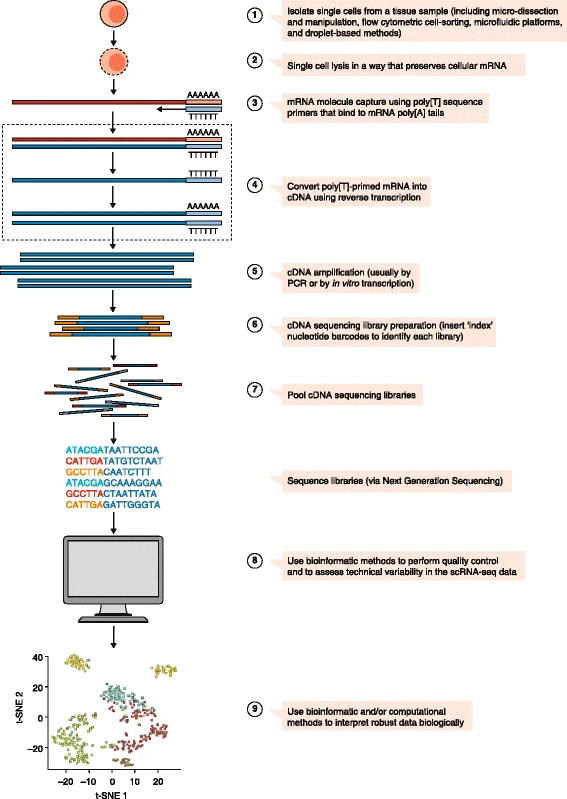
\includegraphics{../figures/scrna_protocol.png}
\end{center}
\caption{General workflow of single-cell RNA-sequencing experiments \citep{scrna_seq}}
\label{fig:SC_RNA}
\end{figure}
\FloatBarrier

\subsection{Quantification of single-cell RNA-seq data}
scRNA-seq data has distinct characteristics that prevent it from being processed by widely used tools developed for bulk RNA-seq data \citep{alevin_fry}. In general, quantification works by aligning the reads generated from the RNA-seq to the reference genome. There are several tools that allow to do that, notably: \emph{STAR} \citep{star}, \emph{kallisto | bustools} \citep{kallisto} and \emph{alevin} \citep{alevin}. However, there is a difference between the first tool and the other two. STAR is an aligner, whereas the other two tools are mapping tools (pseudo-aligners). The difference between an full-aligner and a mapping tool is that the latter does not look for the exact location of the read, as a consequence pseudo-alignment is much faster than full-alignment. Here we focus on \emph{alevin-fry}, and the method we have developed, which will be introduced later, has been built to work on the output of \emph{alevin-fry}.

\section{Objective}

\subsection{RNA velocity}
We investigate spliced and unspliced reads from scRNA-seq data. During transcription, DNA is decoded into precursor messenger RNA (pre-mRNA). Pre-mRNA contains both coding (exons) and non-coding regions (introns). In a next step, introns are removed from the pre-mRNA which leaves only the mature mRNA. Figure \ref{fig:RNA_VELO} shows the process from DNA to mature mRNA, where $\alpha$ is the transcription rate, $\beta$ is the splicing rate and $\gamma$ is the degradation rate.

\begin{figure}[!htb]
\begin{center}
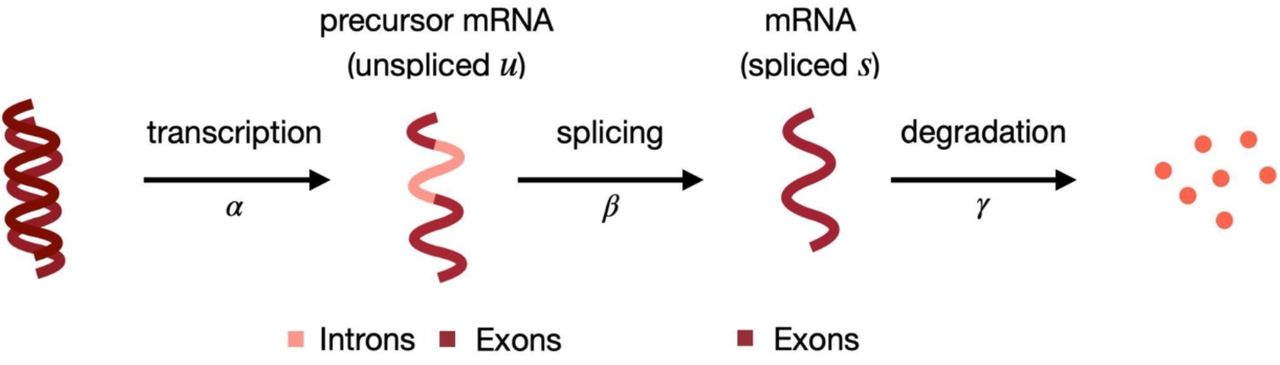
\includegraphics{../figures/regulation.jpg}
\end{center}
\caption{The transcription process from DNA to mature mRNA \citep{rna_velo_traj}}
\label{fig:RNA_VELO}
\end{figure}
\FloatBarrier

It was assumed that there is a signal (RNA velocity) detectable in scRNA-seq data that could reveal the rate and direction of change of an entire transcriptome \citep{rna_velo}. To quantify the relationship between the abundance of pre-mRNA and mature RNA, a simple system of ordinary differential equations was assumed (\ref{eqn:RNA_VELO}): The solution of said system at equilibrium can then easily be estimated and used to explore the regulation of genes:

\begin{equation}
\begin{array}{l}
\frac{du}{dt} = \alpha - \beta u \\
\frac{ds}{dt} = \beta u - \gamma s
\end{array}
\label{eqn:RNA_VELO}
\end{equation}

The derivative of the spliced counts is then defined as the RNA velocity of cells. Thus, the balance of spliced and unspliced counts allows estimating whether a gene is up- or downregulated. If a larger fraction of unspliced counts are present than expected at equilibrium, a gene is likely upregulated. This is because within a short time interval, the newly spliced mRNA will exceed the amount of spliced mRNA which is degraded. Contrarily, if more spliced counts are present at equilibrium than expected, a gene is likely downregulated.

\subsection{Differential regulation}
The abundance of spliced and unspliced reads is directly linked to the regulation of genes and RNA velocities \citep{rna_velo}. Our idea is to examine how the abundance of spliced and unspliced counts changes between experimental conditions and biological replicates. We translate this intuition into the comparison of two experimental conditions, e.g. healthy vs. disease. Following the same intuitive rationale of RNA velocity, if a gene has a higher abundance of unspliced (spliced) counts in group A  compared to group B, then this gene is likely being up-regulated (down-regulated) in group A compared to group B. Thus, we explore the differences in abundance of spliced and unspliced counts to study the differences in regulation between experimental conditions.

If the data contains multiple cell clusters (e.g. cell types), similarly to differential state analyses (\cite{muscat} and \cite{distinct}) we will perform differential analyses in each cluster of cells, hence identifying cell-cluster/cell-type specific changes between conditions. The idea of performing differential analyses on the abundance of spliced and unspliced or exonic and intronic reads is not completely novel as there are at least two other methods that achieve that: \emph{eisaR} and \emph{BRIE2}.

\subsection{Existing methods}

\textbf{eisaR} \citep{eisar_package} is a R package implementation that allows for the split analysis between exons and introns. It allows one to measure changes in mature RNA and pre-mRNA across different experimental conditions. Ultimately, \emph{eisaR} differential testing is based on edgeR \citep{edger_package}. edgeR is a R package that performs differential expression analyses between groups of samples. It implements statistical methods that are based on the negative binomial distribution as a model for count variability. \\

\noindent \textbf{BRIE2} \citep{brie2} is a Bayesian hierarchical model that is implemented in Python and supports the analysis of splicing processes between spliced and unspliced RNA. There are two modes in which the tool can be used. First, the use of differential alternative splicing (DAS), where the aim is to quantify the proportions of alternative splicing isoforms. Second, the use of differential momentum genes (DMG), where the objective is to quantify the proportions of spliced and unspliced RNA in each gene and each cell.

Originally, \emph{eisaR} and \emph{BRIE2} were developed to analyse all cells, but can easily be adapted to perform cell-type specific differential analyses.

\subsection{Mapping uncertainty}
We can identify two main sources of mapping uncertainty concerning spliced and unspliced reads: i) multi-mapping reads across spliced and unspliced versions of a gene, and ii) reads compatible with multiple genes. In fact, it has been shown that many reads (5-40\%) map to multiple genes (\cite{mapping1}, \cite{mapping2}). In our real data analyses (see Section 3), we found approximately 20-30\% of such multi-mapping reads across genes. We additionally found that a significant fraction of reads (6-19\%) are compatible with both S and U versions of a gene. Therefore, the estimated spliced and unspliced counts carry a substantial amount of uncertainty, which should be accounted for in downstream analyses. However, both \emph{eisaR} and \emph{BRIE2} use estimated spliced and unspliced counts and neglect the mapping uncertainty. In this thesis, we propose two approaches that account for said mapping uncertainties.


%%%%%%%%%%%%%%%%%%%%%%%%%%%%%%%%%%%%%%%%%%%%%%%%%%%%%%%%%%%%%%%%%%%%%% 
%%%%%%%%%%%%%%%%%%%%%%%%%%%%%%%%%%%%%%%%%%%%%%%%%%%%%%%%%%%%%%%%%%%%%%

% LaTeX file for Chapter 02


\chapter{Methods} 

\section{DEXSeq}
DEXSeq \citep{dexseq} is a statistical method originally proposed to test for differential exon usage in RNA- seq data, which has been widely adopted in other contexts too, such as differential transcript usage \citep{swimming_downstream}. The model is based on the negative binomial distribution and allows for covariates such as batch effects to be taken into account to offer reliable control of false discoveries \citep{dexseq}. In its original implementation DEXSeq inputs how many reads map to each exon, but the method has alsob been used on transcript level counts. Equation (\ref{eqn:DEXSEQ_A}) shows that the read counts follow a negative binomial distribution where $\alpha$ is the dispersion parameter. Further, a generalized linear model is used to predict the mean via a log-linear link:

\begin{equation}
K_{ijl} \sim \text{NB}(\text{mean}=s_j \mu_{ijl}, \text{dispersion}=\alpha_{il})
\label{eqn:DEXSEQ_A}
\end{equation}

\begin{equation}
log(\mu_{ijl}) = \beta^G_i + \beta^E_{il} + \beta_{i \rho_j}^C + \beta^{EC}_{i \rho_j l}
\label{eqn:DEXSEQ_B}
\end{equation}

where $\text{NB(a, b)}$ denotes the negative binomial distribution with mean a and dispersion b, $s_j$ is .. \\

The dispersion parameter allows to model over-dispersed data (i.e. higher variance than mean). Here, we propose to use DEXSeq on estimated USA counts, and perform a differential usage test between conditions. This models ambiguous reads separately from spliced and unspliced or exonic and intronic, thus eliminating one of the main sources of mapping uncertainty. However, the uncertainty related to reads mapping to multiple genes is still neglected by this approach. 

\section{Differential regulation}
To address both sources of mapping uncertainty we propose our novel method. Similar to the idea above, we implemented a hierarchical Bayesian approach that models ambiguous counts separately from spliced and unspliced. Gene allocation is modeled as a latent state to address the gene-related mapping uncertainty. The model consists of two nested models: First, we use a Dirichlet-multinomial model for the relative abundance of the USA counts in each gene. Second, a multinomial model that models the relative abundance of genes for each sample individually.



%%%%%%%%%%%%%%%%%%%%%%%%%%%%%%%%%%%%%%%%%%%%%%%%%%%%%%%%%%%%%%%%%%%%%%
%%%%%%%%%%%%%%%%%%%%%%%%%%%%%%%%%%%%%%%%%%%%%%%%%%%%%%%%%%%%%%%%%%%%%%

% LaTeX file for Chapter 03


\chapter{Results}

\section{Exploratory Data Analysis}

\subsection{Mouse kidney cells} \label{mouse_dataset}
The first data set stems from a paper that investigates potential cellular targets of kidney disease in mice \citep{mouse_cells}. The authors isolated and sequenced a total of 57'979 cells from whole kidney cell suspensions (one kidney per mouse) derived from seven healthy male mice using droplet-based single-cell RNA sequencing. The samples were labelled as: normal1, normal2, normal3, normal4, Ksp-cre-GFP, Scl-cre-GFP and Pod-cre-GFP. For our work, we decided to use the raw data from the four samples that were labelled as normal to ensure the biological reproducibility between the samples.

We used the \emph{alevin-fry} pipeline to quantify the raw single-cell RNA sequencing data for further use in the R programming environment. Quality control is a crucial stage in data pre-processing as low-quality libraries can contribute to misleading results in downstream analyses \citep{OSCA}. Therefore, we filtered lowly abundant genes and low-quality cells to mitigate said problems to improve interpretability of the results. 

To identify low-quality cells, cell-specific QC metrics were calculated with the \emph{perCellQCMetrics} function from the \emph{scater} R package \citep{scater}. These metrics include the total number of expressed genes, the overall count across all genes, and the fraction of counts assigned to control genes such as mitochondrial genes. By setting a specific threshold on per-cell QC metrics, high-quality cells can be retained. In our setting, outliers are defined as cells with library sizes more than two median absolute deviations away from the median library size. Figure \ref{fig:QC} summarizes the process from unprocessed to processed single-cell experiment. 

\begin{figure}[!htb]
\begin{center}
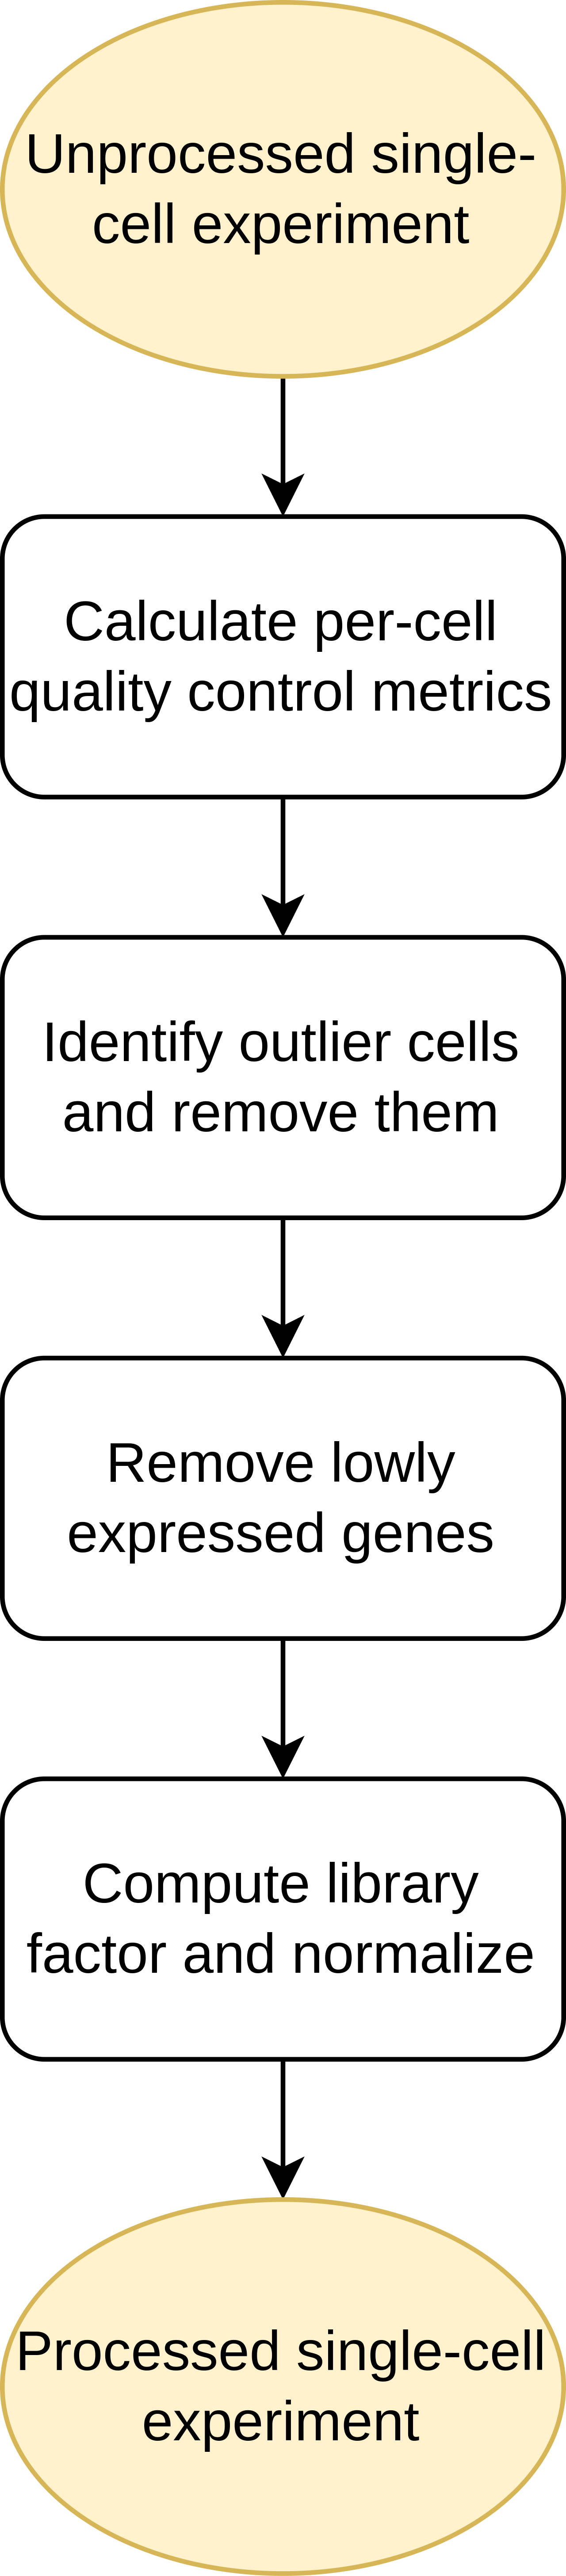
\includegraphics[width=1.5in,height=6in]{figure/qc.png}
\end{center}
\caption{Quality control process from unprocessed, raw to processed, filtered single-cell experiment}
\label{fig:QC}
\end{figure}
\FloatBarrier

After filtering, the data set consists of 23'543 cells and 18'537 genes. Next, we used the \emph{singleR} function from the \emph{singleR} R package \citep{singleR} for cell-type annotation. Cell-type annotation is important to determine what biological state is represented by cell clusters which helps the interpretability of the results and their implications \citep{OSCA}. \emph{singleR} is a method that assigns labels based on the reference samples with the highest Spearman rank correlation while only using marker genes between pairs of labels to focus on the relevant differences between cell types \citep{singleR}. Figure \ref{fig:UMAP_mouse_sample_id} shows the Uniform Manifold Approximation and Projection (UMAP) of the cells coloured by their respective sample id. From Figure \ref{fig:UMAP_mouse_sample_id} one can observe that the projection of the cells is very similar across the samples. Further, Figure \ref{fig:UMAP_mouse_cell_type} also illustrates that cells from the same cell-type cluster together, as one would expect. 

Figure \ref{fig:mouse_cell_type} shows that the annotated cells were largely classified as either: Adipocytes, Epithelial cells and Hepatocytes. Additionally, one can observe that those three cell types are approximately evenly distributed across the four samples. For further analyses we focus on those cell types to investigate the performance of existing methods for the detection of differentially expressed genes and design our own simulation study.

\begin{figure}[!htb]
\begin{center}
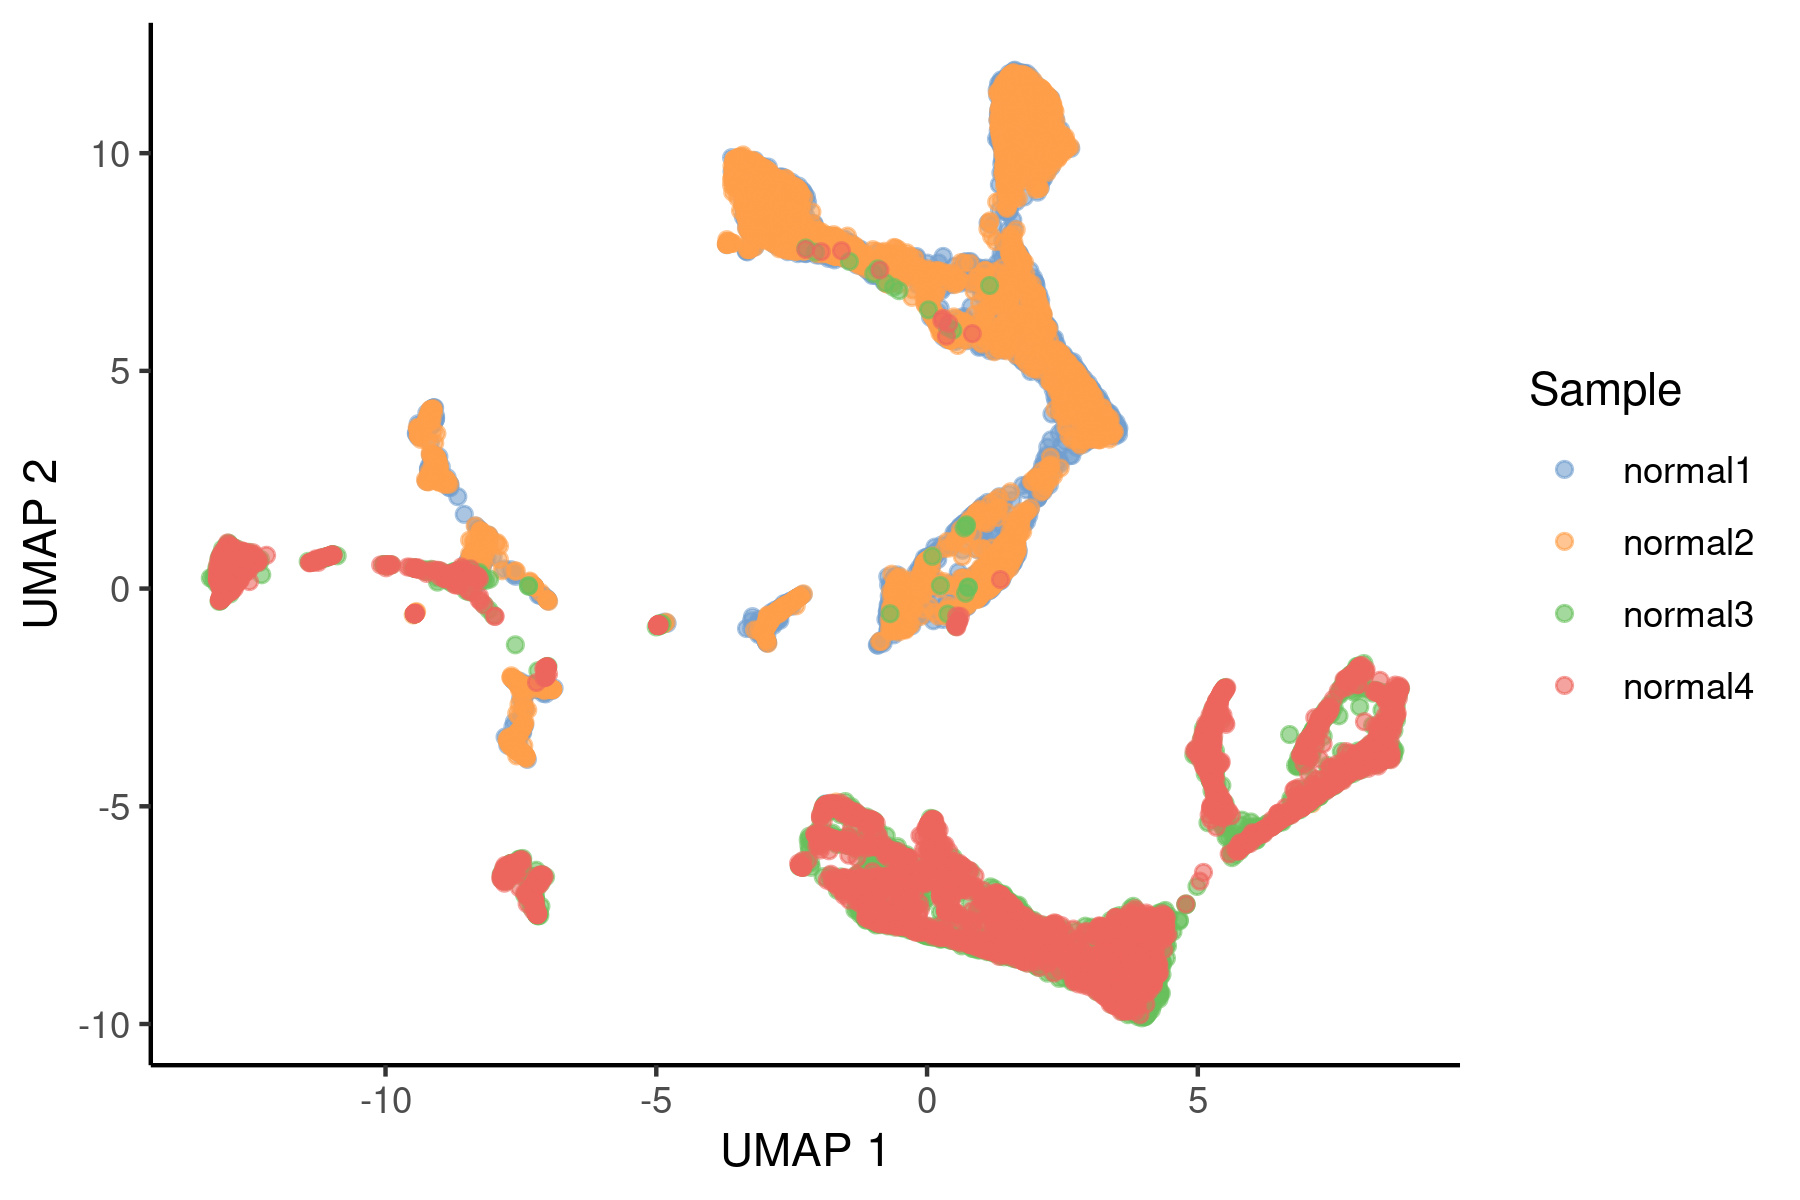
\includegraphics[width=6in,height=4in]{figure/kidney_mouse/UMAP_mouse_sample_id.png}
\end{center}
\caption{UMAP representation of the mouse kidney cells coloured by sample id}
\label{fig:UMAP_mouse_sample_id}
\end{figure}
\FloatBarrier

\begin{figure}[!htb]
\begin{center}
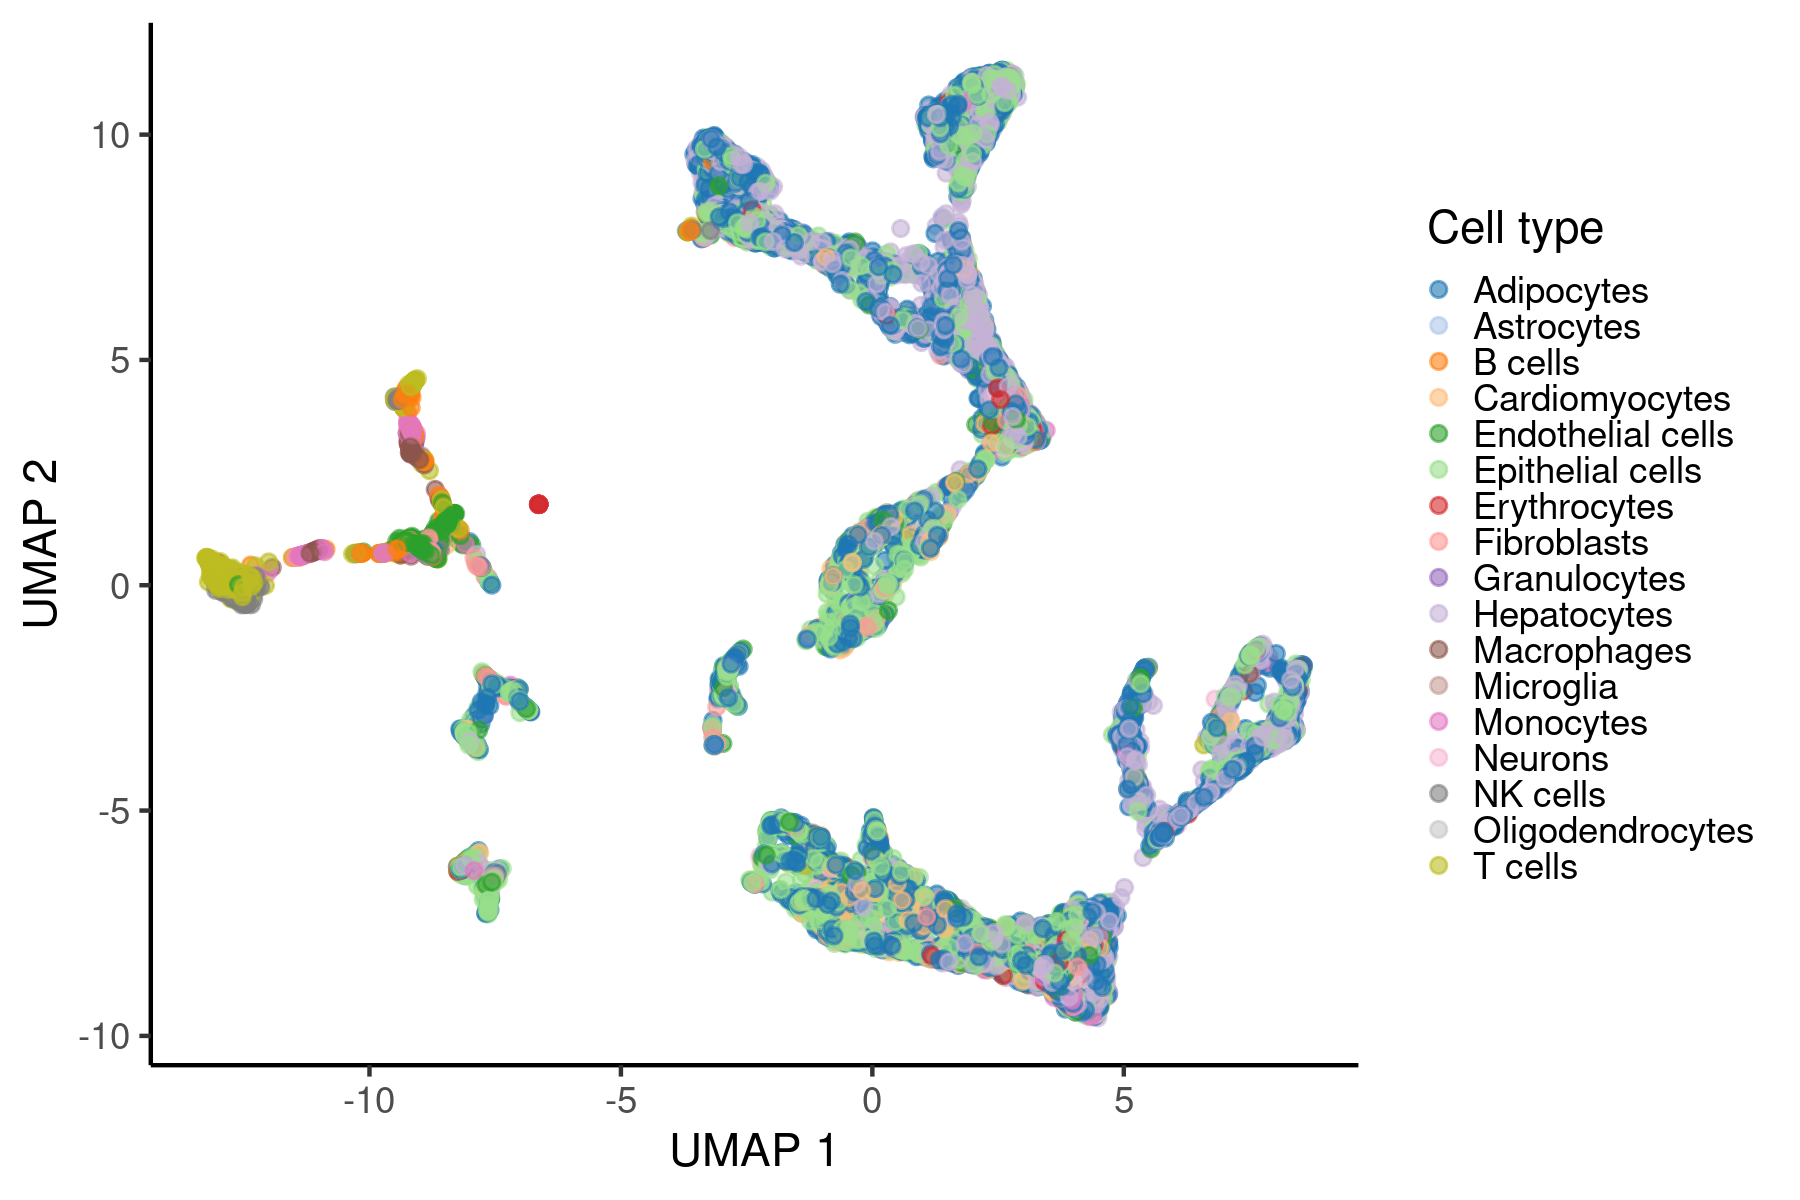
\includegraphics[width=6in,height=4in]{figure/kidney_mouse/UMAP_mouse_cell_type.png}
\end{center}
\caption{UMAP representation of the mouse kidney cells coloured by cell type}
\label{fig:UMAP_mouse_cell_type}
\end{figure}
\FloatBarrier

\begin{figure}[!htb]
\begin{center}
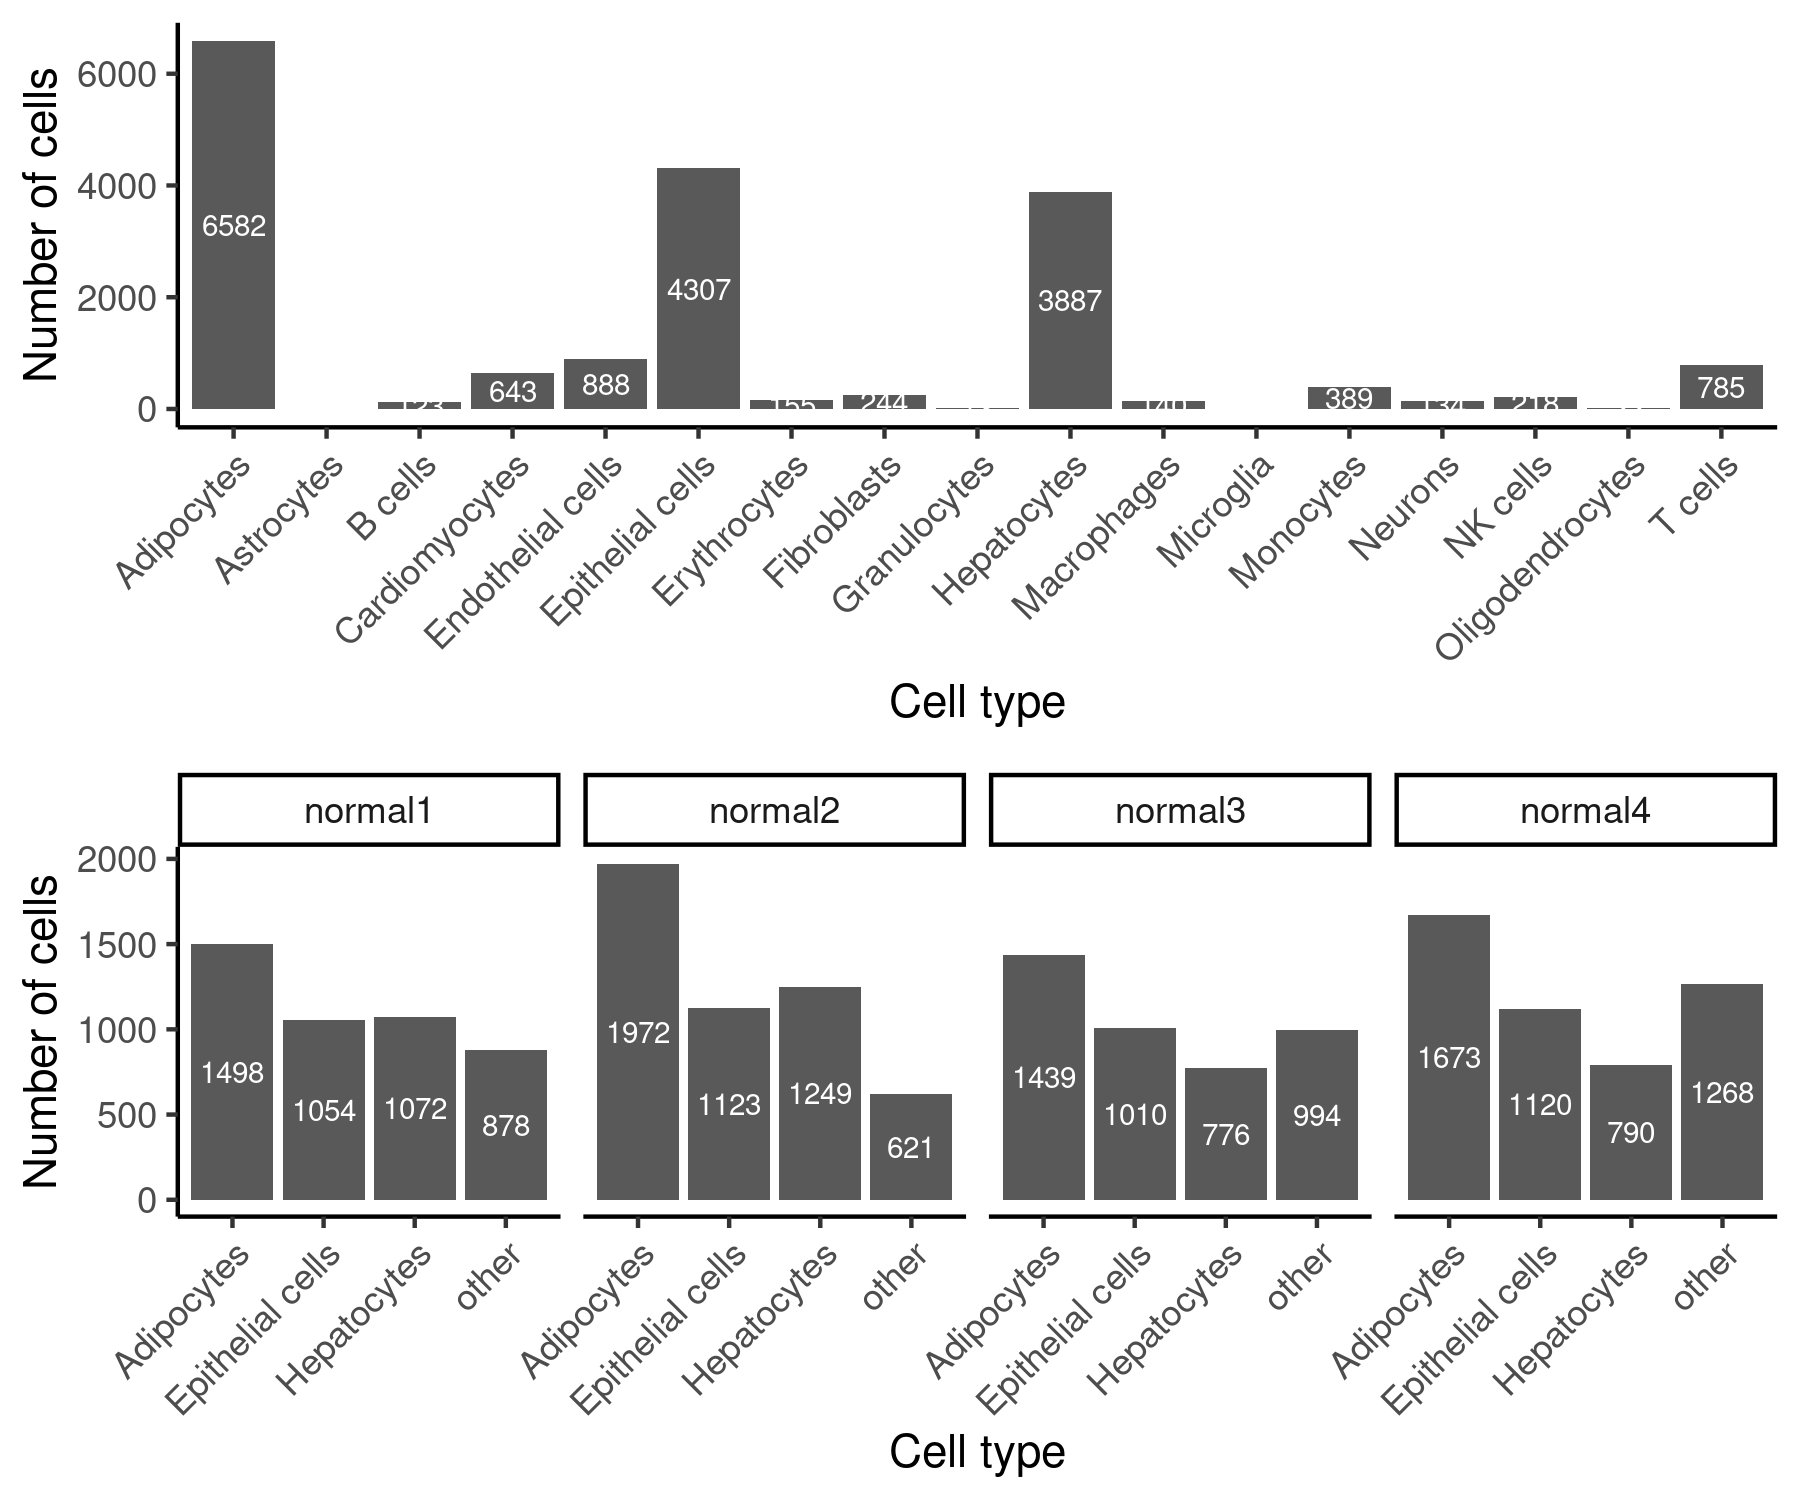
\includegraphics[width=6in,height=5in]{figure/kidney_mouse/cell_type_distribution.png}
\end{center}
\caption{Frequency distribution of the cell types after quality control} 
\label{fig:mouse_cell_type}
\end{figure}
\FloatBarrier

\section{Simulation study}

\subsection{Simulation strategy}
Initially, the simulation strategy was to invert the spliced and unspliced counts for 10\% of genes for all cells that belong to an arbitrary group A. The set of genes whose counts were to be inverted was randomly drawn by a sampling algorithm without replacement (hypergeometric distribution). There are many different ways to introduce a differential effect, however nailing down on inverting the spliced and unspliced counts seemed like a neat way to do this without actually modifying the values. Additionally, differential gene expression was introduced in 10\% of genes in all cells that belong to said arbitrary group A. This was achieved by multiplying the counts (ten-fold gene expression) for 10\% randomly drawn genes in group A. Again, the set of genes was randomly drawn by the same sampling algorithm as before. In this manner two datasets were created, one with and one without differential gene expression. The genes and cells that were subject to change were stored as ground truth for further evaluation in the downstream analyses. Figure \ref{fig:simulation_process} illustrates the simulation process from the original mouse kidney data set to two the simulated data sets. However, these simulations do not yet account for mapping uncertainty. Therefore, the simulation process was enhanced with the use of \emph{minnow} \citep{minnow} in a way that the data now contains mapping uncertainty between spliced and unspliced reads. (GO MORE IN DEPTH BUT WHAT ELSE COULD WE SAY???)

\begin{figure}[!htb]
\begin{center}
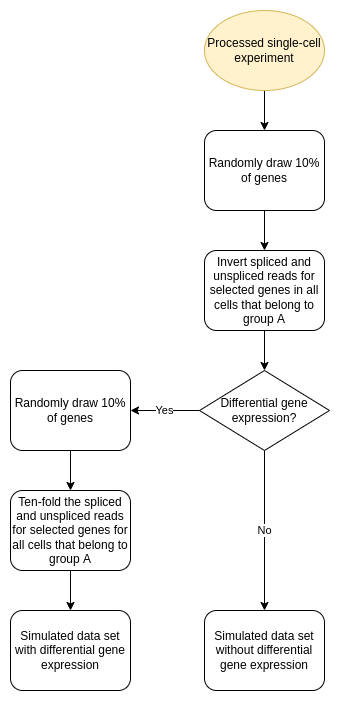
\includegraphics[width=3in,height=6in]{figure/kidney_mouse/first_simulation_process.png}
\end{center}
\caption{Simulation process from original mouse data set to simulated data sets}
\label{fig:simulation_process}
\end{figure}
\FloatBarrier

\subsection{Simulating without Minnow}

\subsection{Simulating with Minnow}

\section{Null data analysis on the mouse kidney data}

\section{Computational benchmark}

\section{Data availability}

\noindent\textbf{Kidney mouse cells} \\
The raw data can be downloaded from NCBI GEO (accession number GSE107585). \\ 
\url{https://www.ncbi.nlm.nih.gov/geo/query/acc.cgi?acc=GSE107585} \\

\section{Code availability}
All code for data preprocessing and analysis associated with the thesis is available at \url{https://github.com/joelmeili/DifferentialRegulation}. Any updates will also be published on GitHub.


%%%%%%%%%%%%%%%%%%%%%%%%%%%%%%%%%%%%%%%%%%%%%%%%%%%%%%%%%%%%%%%%%%%%%%
%%%%%%%%%%%%%%%%%%%%%%%%%%%%%%%%%%%%%%%%%%%%%%%%%%%%%%%%%%%%%%%%%%%%%%

% LaTeX file for Chapter 04


\chapter{Discussion}

\section{Conclusion} 
In this thesis we investigated, how the relative abundance of spliced and unspliced reads differs between experimental conditions. Changes to these relative abundances are directly linked to gene regulation and methods that are capable of detecting these differences already exist (e.g. \emph{BRIE2} and \emph{eisaR}). We identified two main sources of mapping uncertainty: reads mapping to multiple genes, and reads mapping to both spliced and unspliced versions of a gene. We proposed two approaches to deal with these: i) \emph{DEXSeq} on USA estimated counts, which accounts for the first, and \emph{DifferentialRegulation} on the USA-based equivalence classes, which also uses a latent variable model for reads mapping to multiple genes, hence accounting for both sources of mapping uncertainty. We investigated the performance of all methods on two semi-simulated data sets. The semi-simulated data sets were created from real scRNA-seq data with four biological replicates. In a first step, we introduced an arbitrary differential effect to a subset of genes and cells by inverting the counts of spliced and unspliced reads. In one of the two simulations we also added DGE to a second subset of genes and cells as an additional nuisance parameter. Multi-mapping uncertainty was considered next to make the semi-simulated data sets more realistic. This was achieved by simulating, at the read level, with \emph{minnow} and subsequently aligning simulated reads with \emph{alevin-fry}, where we used the two semi-simulated data sets as input for \emph{minnow}. We then analysed the performance of \emph{BRIE2}, \emph{eisaR}, \emph{DEXSeq} and \emph{DifferentialRegulation} in detecting the differential genes by comparing ROC and TPR v. FDR curves. From this analysis we found that \emph{DifferentialRegulation} controls the FDR well for both data sets in comparison to the other three methods. Additionally, we examined the results stratified by gene abundance levels to investigate how robust the methods are to gene abundance with and without DGE. From this analysis we concluded that \emph{DifferentialRegulation} is the only method with good TPR and well calibrated FDR across all levels of gene abundance. Next, we did a null analysis on the original data set where we compared the distribution of p-values for all three possible group separations. We found that \emph{BRIE2} had inflated p-values for all three group separations, whereas \emph{DifferentialRegulation} had no inflated p-values at all. From the null analysis (where no differences between groups are expected) it was also shown that \emph{DifferentialRegulation} seems to be marginally conservative as there was a tendency for inflation towards one. Ultimately, we ran a computational benchmark on the null data where we applied all four methods on all three possible group separations and averaged the runtime. From the computational benchmark it was shown that the better performance of \emph{DifferentialRegulation} comes with a longer runtime, however, there is also the possibility to run the method without equivalence classes, which is slightly less accurate however much faster. From the previous analyses, we show that \emph{DifferentialRegulation} had overall better results than the other methods, however, there are also some caveats to the method, for example, \emph{DifferentialRegulation} cannot deal with additional covariates e.g. batch effects, whereas \emph{BRIE2} and \emph{DEXSeq} can.

\section{Future directions}
\emph{DifferentialRegulation} has already been published on the Bioconductor project, which is an open source software that promotes reproducible analysis of data from emerging biological assays. Further, it is planned to extend the use case of \emph{DifferentialRegulation} from only scRNA-seq data to bulk RNA-seq data, which allows to perform differential analyses at the transcript level. This will enable a double analysis framework: i) identify cell-type specific changes from scRNA-seq data, but at the gene-level due to low transcript resolution, and ii) discover individual differentially regulated transcripts from bulk RNA-seq data, although from an aggregation of cell types. Ultimately, the work of this thesis is part of a future paper which needs some additional analyses on different data sets and some changes to the simulation algorithm.


%%%%%%%%%%%%%%%%%%%%%%%%%%%%%%%%%%%%%%%%%%%%%%%%%%%%%%%%%%%%%%%%%%%%%%
%%%%%%%%%%%%%%%%%%%%%%%%%%%%%%%%%%%%%%%%%%%%%%%%%%%%%%%%%%%%%%%%%%%%%%

\addtocontents{toc}{\protect \vspace*{10mm}}
\addcontentsline{toc}{chapter}{\bfseries Bibliography}

\bibliographystyle{mywiley}
\bibliography{biblio}

\cleardoublepage

\end{document}

%%% Local Variables:
%%% ispell-local-dictionary: "en_US"
%%% End: